\documentclass{article}
\usepackage[latin1]{inputenc}
\usepackage{tikz}
\usetikzlibrary{shapes,arrows,calc}

\newcommand{\circular}[2]{
\node (0) at (0,0){};
\xdef\Radious{#2}
\foreach \nodetext[count=\i] in {#1} {
\xdef\totalIt{\i}
}
\foreach \nodetext[count=\i] in {#1} {
\pgfmathsetmacro\myprev{int{\i-1}}
\pgfmathsetmacro\curxdispl{cos(90-360/\totalIt*(\i-1))*\Radious}
\pgfmathsetmacro\curydispl{sin(90-360/\totalIt*(\i-1))*\Radious}
\path  ($(\curxdispl cm,\curydispl cm)$) node[block,anchor=center] (\i) {\nodetext};
}

\foreach \nodetext[count=\i] in {#1}{
\pgfmathsetmacro\mynext{\ifnum\i<\totalIt int(\i+1)\else 1\fi}
\path[draw,-latex] (\i) to[bend left] (\mynext);
}
}

\begin{document}
\pagestyle{empty}

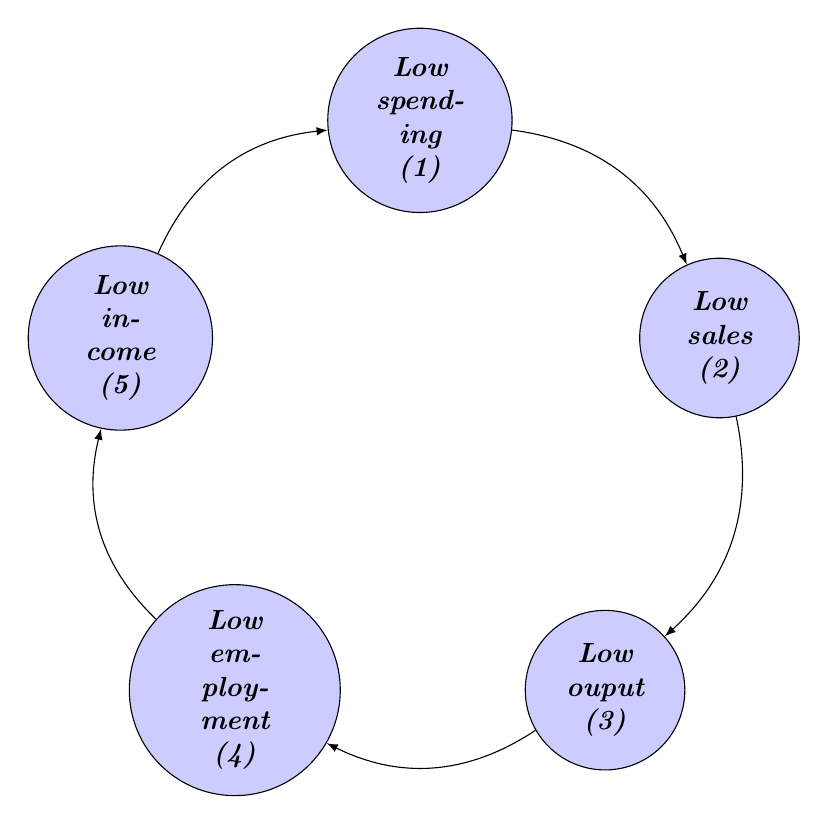
\begin{tikzpicture}
\tikzstyle{block} = [circle, draw, fill=blue!20, 
text width=3.5em, text centered, rounded corners, minimum height=2em]
\circular{\textit{\textbf{Low spending (1)}},\textit{\textbf{Low sales (2)}},\textit{\textbf{Low ouput (3)}},\textit{\textbf{Low employment (4)}},\textit{\textbf{Low income (5)}}}{4}
\end{tikzpicture}
\end{document}

